Il \textbf{QoS (quality of service)} è un indicatore di qualità utilizzato per misurare il livello del servizio, confrontandolo alle aspettative dell'utente.
Il QoS viene associato ai servizi di rete e i flussi generati da essi.
Può essere definito in termini di misure di prestazioni:
\begin{itemize}
	\item Banda disponibile
	\item Ritardo
	\item Perdita di pacchetti
	\item Probabilità di blocking
	\item Ritardo di setup
	\item \ldots
\end{itemize}
Il QoE (quality of experience) è legato al QoS, ma mentre QoS è un indicatore oggettivo, il QoE è un indicatore soggettivo, che dipende dalle aspettative dell'utente.
Possiamo definire un QoS in termini:
\begin{itemize}
	\item \textbf{Assoluti}: definiamo dei parametri numerici che devono essere rispettati, ad esempio: ritardo $< 100$ ms, banda $> 1$ Mbps, \ldots
	\item \textbf{Relativi}: definiamo come il traffico o classe di servizi viene trattato rispetto ad altri.
\end{itemize}
Ricordiamoci che le reti IP sono \textbf{best effort}, quindi non garantiscono alcun QoS.
Le reti best effort hanno successo perché sono semplici, ma negli ultimi anni il bisogno di garanzie di qualità in reti IP è aumentato molto. 
Questo fenomeno ha portato la creazione di numerose nuove soluzioni per garantire la qualità (ad esempio: IntServ, DiffServ, MPLS, \ldots).
Un altro aspetto fondamentale del traffico su reti IP è che è \textbf{bursty}, ovvero ha periodi di alta attività seguiti da periodi di bassa attività.
\\
Possiamo definire almeno due classi di servizi:
\begin{itemize}
	\item \textbf{Servizi real time}: molto sensibili al ritardo, ma non alla perdita di pacchetti, ad esempio: VoIP, video streaming, \ldots
	\item \textbf{Servizi elastici}: molto sensibili alle perdite di pacchetti, ma non al ritardo. Tendenzialmente richiedono ACK per verificare la corretta ricezione dei pacchetti, ad esempio: email, file transfer, \ldots
\end{itemize}
I diversi tipi di servizi richiedono diversi livelli di QoS, e quindi è necessario implementare meccanismi per garantire questi livelli di qualità.
\section{Metodi per la garanzia di QoS}
Per poter garantire il QoS, è necessario implementare almeno un sottoinsieme dei seguenti meccanismi:
\begin{enumerate}
	\item Identificazione del flusso/traffico (etichette)
	\item Progettazione del traffico per stabilire cammini desiderati nella rete (MPLS).
	\item Call admission control (CAC), meccanismi che possono rifiutare una richiesta se non ci sono sufficienti risorse o non è possibile garantire il QoS richiesto per gli altri servizi.
	\item Network resource signalling, meccanismi che permettono di comunicare alla rete le risorse necessarie per un certo servizio. Utili per prendere buone decisioni in CAC.
	\item Meccanismi di regolazione del traffico: si assicurano per il traffico ammesso rispetti gli accordi e non sovraccarichi la rete.
	In caso ciò non valesse, vengono prese delle contromisure.
	\item Tecniche di scheduling per prioritizzare il traffico all'interno dei dispositivi di rete.
	\item Over-provisioning, ovvero fornire più risorse di quelle necessarie per garantire il QoS, in modo da avere un margine di sicurezza.
\end{enumerate}
\section{Regolazione del traffico}
Un provider esterno deve garantire dei servizi con un certo livello di qualità.
Per farlo, stipula due contratti con il cliente:
\begin{itemize}
	\item \textbf{SLA (service level agreement)}: è un contratto tra il provider e il cliente che definisce i livelli di servizio garantiti, ad esempio: banda minima, ritardo massimo, \ldots
	\item \textbf{TCA (traffic conditioning agreement)}: è un contratto che definisce le regole per il traffico generato dal cliente, ad esempio: limiti di banda, politiche di shaping, \ldots
\end{itemize}
\subsection{Service level agreement}
Il SLA è un contratto che definisce i livelli di servizio garantiti dal provider al cliente.
Viene definito basandosi su dei parametri misurabili (metriche), ad esempio:
\begin{itemize}
	\item Banda minima garantita
	\item Ritardo massimo
	\item Perdita di pacchetti massima
	\item \ldots
\end{itemize}
Include diversi \textbf{SLO} (service level objective), che sono obiettivi specifici per ogni parametro in un certo time horizon, ad esempio: 99\% di disponibilità su 1 anno.
\subsection{Traffic conditioning agreement}
Lo sforzo del provider per garantire il SLA dipende dal traffico generato dal cliente, quindi è necessario definire delle regole per il traffico generato dal cliente, in modo da poter garantire il QoS.
Il TCA definisce i profili di traffico dell'utente.
Imposta dei parametri che caratterizzano il traffico generato dall'utente per il quale il provider deve rispettare i SLA.
Il traffico TCA-compliant viene chiamato \textbf{in-traffic} (o compliant), mentre il traffico che non rispetta i parametri definiti nel TCA viene chiamato \textbf{out-traffic} (o non compliant).
Il TCA può includere molti parametri, ad esempio:
\begin{itemize}
	\item Traffico massimo generato (peak rate)
	\item Traffico medio generato (average rate)
	\item Lunghezza dei burst massima
	\begin{itemize}
		\item Numero massimo di pacchetti consecutivi trasmessi al peak rate.
		\item In alternativa, il tempo massimo per il quale il trasmittente può trasmettere al peak rate.
	\end{itemize}
	\item Lunghezza massima del pacchetto
	\item Lunghezza minima del pacchetto
\end{itemize}
\section{Trattamento del traffico}
Accettare il traffico non compliant è rischioso, perché potrebbe sovraccaricare la rete e compromettere la capacità di garantire i SLA.
Il traffico non compliant può essere trattato in diversi modi:
\begin{itemize}
	\item \textbf{Policing}: il traffico non compliant viene scartato.
	\item \textbf{Shaping}: il traffico non compliant viene ritardato, in modo da renderlo compliant.
	\item \textbf{Marking}: il traffico non compliant viene marcato, in modo da poter essere trattato diversamente all'interno della rete (ed eventualmente eliminato se necessario).
\end{itemize}
Il traffico viene analizzato da un regolatore, che decide se è compliant o non compliant, e in caso non lo sia, decide come trattarlo (policing, shaping, marking).
Il regolare inoltre adotta specifici algoritmi per garantire i parametri definiti nel TCA.
Vedremo ora alcuni algoritmi.
\subsection{Token bucket}
Token bucket è un algoritmo usato dal regolatore per controllare i parametri definiti nel TCA, per discriminare il traffico.
I parametri che vengono controllati sono:
\begin{itemize}
	\item Peak rate $p = [\frac{\text{bit}}{\text{s}}]$
	\item Average rate $r = [\frac{\text{bit}}{\text{s}}]$
	\item Lunghezza di burst $L = [\text{s}]$
\end{itemize}
\begin{figure}[H]
	\centering
	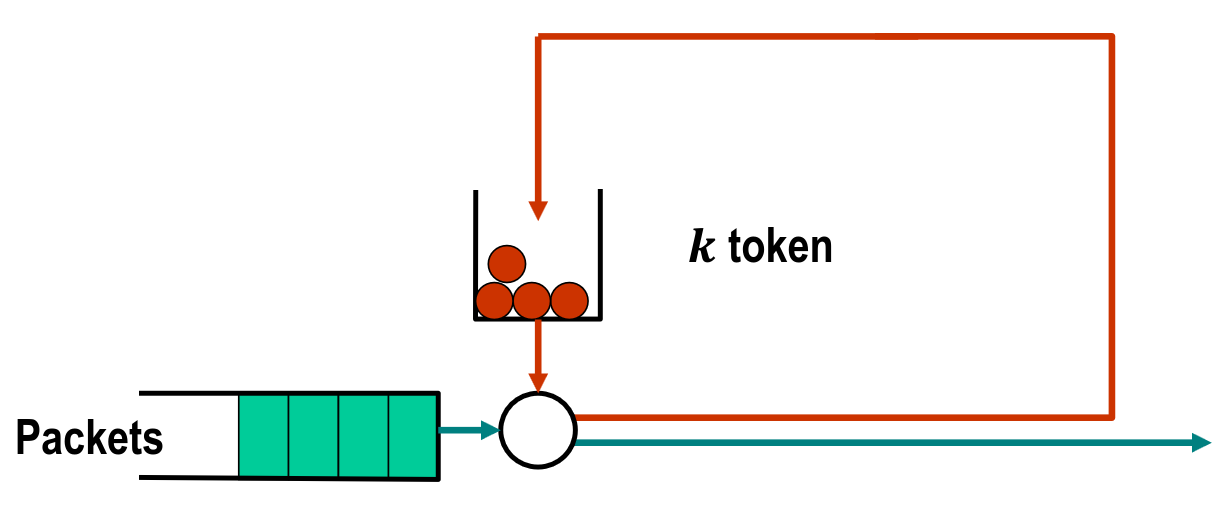
\includegraphics[width=0.8\textwidth]{pictures/5/token_bucket.png}
	\caption{Token bucket}
\end{figure}
\subsubsection{Policing}
Il policer mantiene un serbatoio di token, con capacità massima $k$ di unità di traffico.
Questa capacità può essere espressa in bit, pacchetti, \ldots
Non esiste un buffer per il traffico di input.
Il buffer di token viene riempito a una velocità costante ogni $1/r$ secondi, dove $r$ è il token rate.
Il regolatore ammette il passaggio di un'unità di traffico solo se il serbatoio contiene almeno un token, in questo caso viene rimosso un token dal serbatoio.
Se il serbatoio è vuoto, il traffico viene scartato.
\subsubsection{Shaping}
Lo shaper funziona in maniera simile al policer.
Quando una unità di traffico arriva, se il serbatoio contiene almeno un token e il buffer di traffico è vuoto, allora il traffico viene trasmesso immediatamente e viene rimosso un token dal serbatoio.
Se invece il buffer di traffico non è vuoto e/o il serbatoio è vuoto, allora il traffico viene messo in coda nel buffer di traffico.
Quando il buffer di input non è vuoto, l'unità di traffico viene trasmessa solo quando il serbatoio contiene almeno un token.
\subsubsection{Average e peak rate}
Il peak rate $p$ indica il tasso massimo al quale il traffico può essere trasmesso.
Tipicamente corrisponde alla velocità di trasmissione del link.
Il token rate $r$ e la dimensione del serbatoio $k$ influenzano il tasso medio del traffico $b$.
Un valore di $k$ più grande permette di trasmettere a un peak rate $p$ per un periodo di tempo più lungo, dunque $b$ aumenta.
Un valore di $r$ più grande permette di trasmettere a un tasso più alto quando il serbatoio è vuoto, dunque $b$ aumenta.
Ovviamente $b < p$. 
\subsubsection{Traffico bursty}
Il serbatoio di credito permette al traffico generato dalla sorgente di essere ammesso nella rete a una velocità maggiore del token rate $r$ (peak rate $p$).
Assumiamo che $p >> r$ e che il traffico generato dalla sorgente sia bursty, ovvero abbia periodi di alta attività seguiti da periodi di bassa attività.
Il token bucker preserva la burstiness del traffico.
Il regolatore controlla la lunghezza massima del burst $L$, calcolata come $L=\frac{k}{p-r}$.
L'average rate $b$ viene indirettamente controllato modificando $L$ (che dipende da $K$ e $r$).
\subsubsection{Funzione di restrizione}
Il regolatore implementa una funzione di restrizione, viene creata una retta $f(t)=k+rt$ che indica il numero massimo di unità di traffico compliant che sono state lasciare passare.
Al tempo $\overline{t}$ sono state fatte passare al più $f(\overline{t})$ unità di traffico compliant.
Il traffico in eccesso viene considerato come non compliant e trattato di conseguenza (policing, shaping, marking).
Il policer scarta il traffico non compliant, causando un ritardo risibile ma con una perdita di pacchetti.
Lo shaper mantiene il traffico non compliant in un buffer e lo serve appena sono disponibili dei token. Lo shaper non ha perdita di pacchetti ma introduce un ritardo significativo.
Il marker non scarta il traffico non compliant, ma lo marca in modo da poter essere trattato diversamente all'interno della rete (ad esempio: scartato se necessario).
\subsection{Leaky bucket}
Algoritmo alternativo al token bucket, che non presenta un serbatoio di token.
Un credito viene generato ogni $1/r$ unità di tempo.
Tipicamente il buffer di input ha capacità finita $B$, quando il buffer è pieno, il traffico in eccesso viene scartato.
Il regolatore ammette il passaggio di una unità di traffico ogni $1/r$ unità di tempo.
Dato che i crediti non possono essere accumulati, qualsiasi traffico bursty viene smussato, nel senso che non è possibile trasmettere a un tasso maggiore di $r$.
\section{Allocazione delle risorse}
Le tecniche di policing, shaping e marking permettono di migliorare l'allocazione delle risorse di rete.
Quando diversi flussi vengono multiplexati per generare un singolo output aggregato, le risorse devono essere allocate in maniera intelligente.
Ci sono due tipi di allocazione delle risorse:
\begin{itemize}
	\item \textbf{Allocazione deterministica}: le risorse vengono divise in modo statico tra i diversi flussi in ingresso. Non c'è perdita di pacchetti se il sistema è ben progettato.
	\item \textbf{Allocazione statistica}: le risorse vengono divise in modo dinamico tra i diversi flussi in ingresso, basandosi sulle loro esigenze. C'è una certa probabilità di perdita di pacchetti, ma si ottiene una maggiore efficienza nell'utilizzo delle risorse.
\end{itemize}
Ora ci concentreremo sull'allocazione deterministica.
\subsection{Peak allocation}
Per evitare perdite, questa tecnica viene utilizzata quando il traffico in ingresso non è stato regolato da nessun regolatore.
A ogni flusso viene assegnata una porzione della capacità $C$ del link di uscita uguale al suo peak rate $p [\text{bit}/\text{s}]$.
Assumendo che i flussi siano omogenei, quindi abbiano lo stesso peak rate $p$, allora il numero massimo di flussi che possono essere supportati senza perdita è $N_p =  \frac{C}{p} $.
Se $b_{\text{avg}}\leq p$ è il tasso medio di ogni flusso, allora possiamo definire l'\textbf{efficienza} della strategia di allocazione come $\eta_p = \frac{N_p \cdot b_{\text{avg}}}{C}=\frac{b_{\text{avg}}}{p}$.
Questa strategia considera il peggior caso possibile, maggiore è la differenza tra il tasso massimo e medio peggiore è l'efficienza.
D'altro canto, è garantita l'assenza di perdite.
\subsection{Dual leaky bucket allocation}
Possibile quando il traffico di ingresso è stato regolato da token bucker o leaky bucket, anche in cascata.
Una sorgente viene modellata da tre parametri:
\begin{itemize}
	\item $r_s$: token rate
	\item $B_{ts}$: dimensione del serbatoio di token
	\item $p_s>r_s$: peak rate
\end{itemize}
La durata massima dei burst viene ridotta a un valore ben determinato.
Questo permette di allocare in maniera deterministica e lossless se i parametri $B$ e $C$ vengono opportunamente scelti, dove 
$B$ è la dimensione del buffer del multiplexer e $C$ è la capacità del link di uscita.
Il primo elemento (TB) regola il tasso di output $r_s$ con una certa tolleranza $B_{ts}$.
Il secondo elemento (LB) regola il peak rate $p_s<p$ dove $p$ è la capacità del link di uscita.
Dunque DLP impone un limite sulla quantità massima di tempo al quale i pacchetti possono essere ammessi al peak rate di rete $p_s$
$T_{\text{peak}}=L=\frac{B_{ts}}{p_s-r_s} [\text{s}]$.
\\
Obiettivo: se $N_{\text{DLB}}$ è il numero massimo di flussi in ingresso regolati da un DLB e ammessi nella rete senza perdite, esprimerlo come funzione dei parametri del DLB, cioè $r_s$, $p_s$, $B_{ts}$.
\begin{itemize}
\item Assunzione 1: i flussi emessi dalle sorgenti sono tutti regolati considerando gli stessi parametri DLB.
\item Assunzione 2: la stessa porzione di capacità/buffer di uscita $(c,b)$ del multiplatore è assegnata a ciascun flusso, come frazione di $C$, $B$.
\end{itemize}
Dando per assunte 1 e 2, abbiamo che $B = N_{\text{DLB}}b$ e $C = N_{\text{DLB}}c$.
Devono essere soddisfatte due condizioni per garantire un ritardo massimo ai pacchetti e evitare perdite:
\begin{enumerate}
\item Definizione di una dimensione appropriata del buffer $B$ data una massima latenza accettabile $D_{\max}$ aggiunta dal multiplatore a un pacchetto di un qualsiasi flusso:
\[
D_{\max} = \frac{B}{C} = \frac{N_{\text{DLB}}b}{N_{\text{DLB}}c} = \frac{b}{c} [\text{s}] \rightarrow B = C \cdot D_{\max}
\]
\item Allocazione di un'appropriata porzione di buffer $b$ per ogni flusso, data la massima durata del burst $T_{\text{peak}}$ e considerando una porzione allocata di banda $c < p_s$, per evitare perdite:
\[
b = (p_s - c)\,T_{\text{peak}} \ [\text{bit}]
\]
\noindent
Moltiplicando entrambi i termini per $N_{\text{DLB}}$, la condizione può essere riscritta come:
\[
N_{\text{DLB}}b = N_{\text{DLB}}(p_s - c)T_{\text{peak}}
\]
\[
N_{\text{DLB}}b = (N_{\text{DLB}}p_s - N_{\text{DLB}}c)T_{\text{peak}}
\]
\[
B = (N_{\text{DLB}}p_s - C) T_{\text{peak}}
\]
\end{enumerate}
e considerando il sistema di equazioni:
\[
\begin{cases}
B = C \cdot D_{\max} \\
B = (N_{\text{DLB}}p_s - C)T_{\text{peak}}
\end{cases}
\]
è possibile calcolare $N_{\text{DLB}}$:
\[
N_{\text{DLB}} = \frac{C}{p_s}\left(1 + \frac{D_{\max}}{T_{\text{peak}}}\right)
= \frac{C}{p_s}\left(1 + \frac{D_{\max}(p_s-r_s)}{B_{ts}}\right)
\]
Regolando opportunamente i parametri $p_s$, $r_s$ e $B_{ts}$ per ciascuna sorgente, è possibile ottenere valori diversi di $N_{\text{DLB}}$.
L'azione viene effettuata alle sorgenti!
\subsection{Confronto tra peak allocation e dual leaky bucket}
Numero massimo di flussi con peak allocation
\[
N_p = \frac{C}{p}
\]
Numero massimo di flussi con allocazione DLB
\[
N_{\text{DLB}} = \frac{C}{p_s}
\left(1 + \frac{D_{\max}}{T_{\text{peak}}}\right)
\]
Poiché $p > p_s$, vale che
\[
N_{\text{DLB}} > N_p
\]
Questo significa che il DLB rende possibile multiplexare più flussi senza perdite rispetto a una strategia di peak allocation.
\section{Scheduling}
Le tecniche di scheduling permettono di partizionare le interfacce di usicta del router tra i vari flussi di traffico.
La banda è condivisa tra i pacchetti in diverse code. Uno scheduler determina come la banda viene partizionata.
Vi sono diversi possibili approcci.
\subsection{Time division multiplexing}
Per ogni turno di tempo, viene creata una coda.
\begin{figure}[H]
	\centering
	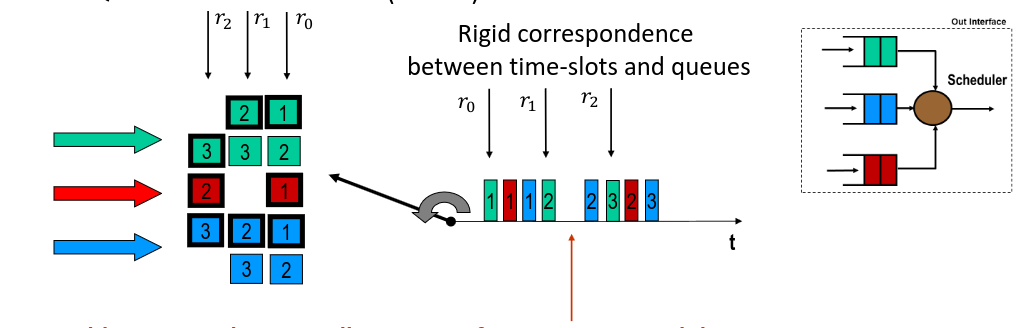
\includegraphics[width=0.8\textwidth]{pictures/5/tdm.png}
	\caption{Time division multiplexing}
\end{figure}
Questa strategia non permette di riusare le risorse inutilizzate quando una coda è vuota.
\subsection{Round Robin (fair queuing)}
La banda viene partizionata in modo dinamico, trasmettendo ciclicamente un pacchetto per coda (se presente).
\begin{figure}[H]
	\centering
	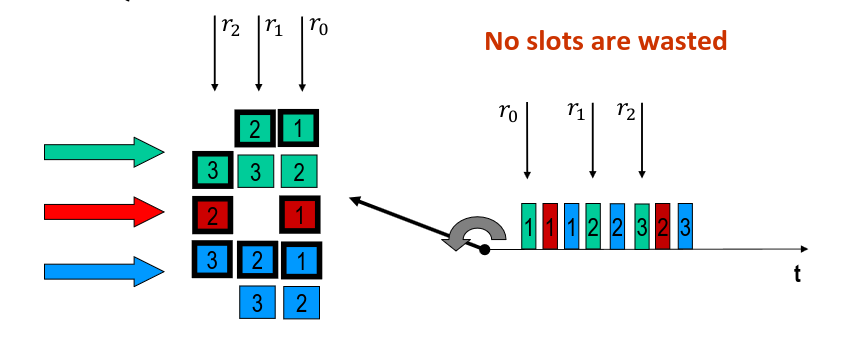
\includegraphics[width=0.8\textwidth]{pictures/5/rr.png}
	\caption{Round Robin}
\end{figure}
\subsection{Weighted Fair Queuing}
La banda viene partizionata in modo dinamico e proporzionale.
Vengono trasmessi al massimo $K_i$ pacchetti per ogni coda $i$, in modo pseudo-ciclico.
\begin{figure}[H]
	\centering
	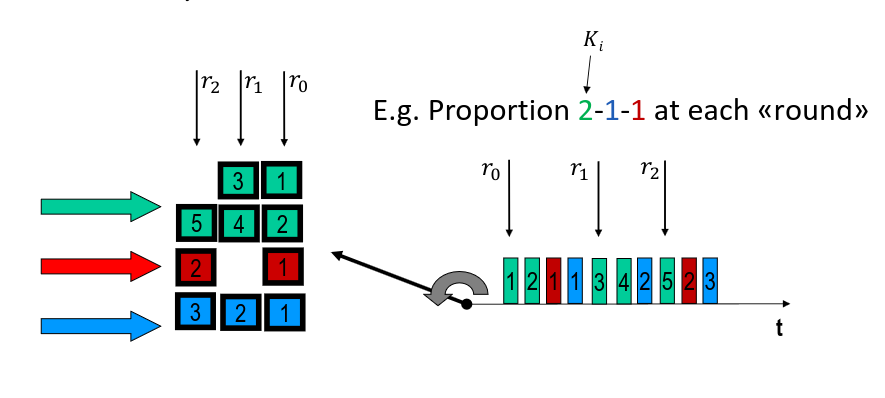
\includegraphics[width=0.8\textwidth]{pictures/5/wfq.png}
	\caption{Weighted Fair Queuing}
\end{figure}
\subsection{Service priority}
Partizionamento dinamico basato sulle priorità.
\begin{figure}[H]
	\centering
	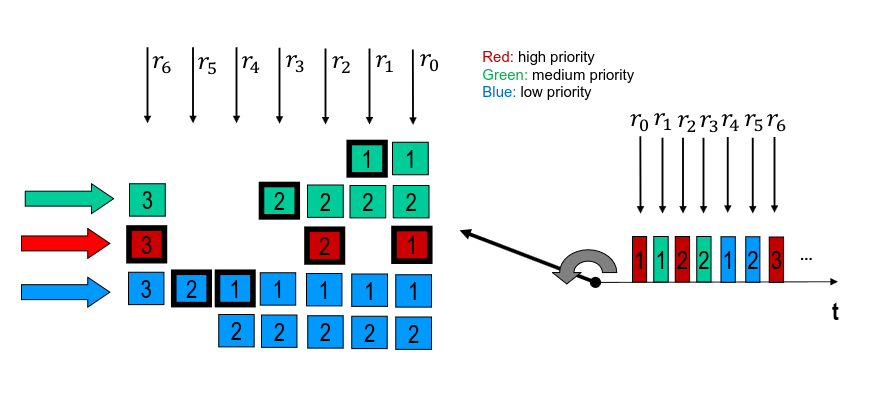
\includegraphics[width=0.8\textwidth]{pictures/5/sp.png}
	\caption{Service priority}
\end{figure}
Le code con priorità bassa potrebbero soffrire di ritardi significativi.
Se i pacchetti a priorità inferiore da trasmettere sono lunghi, altri pacchetti a priorità più alta nelle code rischiano di essere ritardati.
\begin{itemize}
\item Esempio: Rosso ha alta priorità, Verde ha priorità media.
\item Effetto di un pacchetto verde lungo (1) e di due verdi di lunghezza dimezzata (2).
\end{itemize}
\begin{figure}[H]
	\centering
	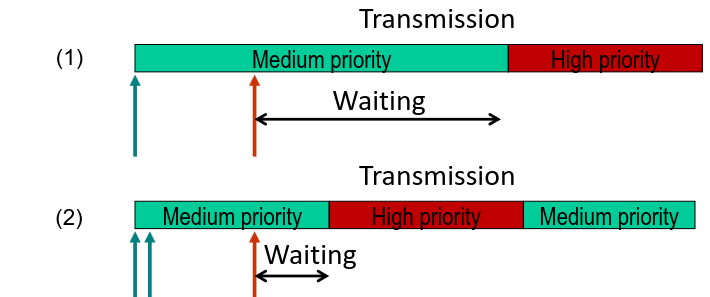
\includegraphics[width=0.6\textwidth]{pictures/5/priority.png}
	\caption{Effetto di un pacchetto lungo a priorità media}
\end{figure}
Questo porta a dover frammentare i pacchetti, specialmente su reti lente.
\subsubsection{Modalità di frammentazione}
I pacchetti IP potrebbero essere frammentati su connessioni lente.
In questo modo, però, il livello IP è in grado di ricomporli solo al ricevitore.
La presenza di un gran numero di frammenti IP nella rete porta a forti inefficienze.
I meccanismi di frammentazione a livello 2 vengono adottati su connessioni point-to-point lente (ad esempio PPP, Point-to-Point Protocol).
La ricomposizione avviene all'altro capo del collegamento point-to-point.
\section{Call admission protocol}
Set di azioni intraprese da una rete durante l'istituzione o la rinegoziazione di una connessione. Obiettivo: (1) determinare se la richiesta di connessione può essere accettata e (2) allocare le risorse per il flusso correlato sul percorso scelto.
\\
È garantito che, per ogni link o nodo sul percorso seguito dal flusso, siano assegnati:
\begin{enumerate}
	\item Una porzione della capacità del link (assegnazione di banda).
	\item Una porzione del buffer (cioè, coda) nell'interfaccia di uscita del nodo (assegnazione di buffer).
\end{enumerate}
\bigskip
La quantità di banda e buffer allocati dipende dai requisiti di QoS.
\\
L'entità che esegue la procedura CAC deve conoscere:
\begin{itemize}
	\item La quantità di risorse richieste per soddisfare adeguatamente la richiesta.
	\item La quantità di risorse attualmente utilizzate su ogni link/nodo.
\end{itemize}

In altre parole, deve:
\begin{enumerate}
	\item Verificare se esiste un percorso con tale disponibilità.
	\item Riservare le risorse se così.
\end{enumerate}
\bigskip
Ci sono tre modalità per eseguire la procedura CAC:
\begin{itemize}
	\item \textbf{Modalità centralizzata}: il CAC è eseguito da un server centrale.
	\item \textbf{Modalità distribuita}: ogni nodo nella rete contribuisce al CAC.
	\item \textbf{Modalità ibrida}: il CAC è eseguito solo ai nodi di bordo della rete.
\end{itemize}
\subsection{Modalità centralizzata}
Il CAC è eseguito da un server centrale, che riceve tutte le richieste e conosce tutte le informazioni necessarie per prendere decisioni appropriate.
\\
\textbf{Vantaggi:}
\begin{itemize}
	\item Il signalling verso i nodi è semplice.
	\item Il percorso ottimale può essere determinato.
\end{itemize}
\textbf{Svantaggi:}
\begin{itemize}
	\item Problemi di scalabilità e affidabilità.
	\item Non ben tollerato da IP, eccetto per sistemi molto semplici: la procedura CAC deve essere in grado di decidere il percorso di routing ottimale e ignorare le decisioni fatte dai protocolli di routing standard.
\end{itemize}
Di conseguenza, viene utilizzato esclusivamente in sistemi di reti piccole.
\subsection{Modalità distribuita}
Ogni nodo è consapevole delle sue risorse di rete occupate e contribuisce al CAC.
\\
\textbf{Vantaggi}
\begin{itemize}
	\item Sistema robusto e affidabile.
\end{itemize}
\textbf{Svantaggi}
\begin{itemize}
	\item Sistema complesso, dove il sistema di signalling è necessario per:
	\begin{itemize}
		\item Raccogliere informazioni sull'occupazione delle risorse da altri nodi.
		\item Riservare le risorse sul percorso (ad es. Resource ReSerVation Protocol, RSVP, RFC 2210).
	\end{itemize}
\end{itemize}

\subsection{Modalità ibrida}
Il CAC è eseguito dai router ai bordi della rete (router di confine):
\begin{itemize}
	\item Questi router periodicamente ottengono informazioni sullo stato delle risorse di rete (anche dai router core) e prendono decisioni.
\end{itemize}\noindent
\textbf{Vantaggi}
\begin{itemize}
	\item Sistema meno complesso rispetto alla modalità distribuita: meno nodi coinvolti nella procedura CAC.
\end{itemize}
\textbf{Svantaggi}
\begin{itemize}
	\item Anche in questo caso è necessario: un sistema di signalling per raccogliere periodicamente lo stato dell'occupazione delle risorse da altri nodi; un sistema di signalling per riservare le risorse di rete (RSVP).
\end{itemize}

\section{Integrated Services (IntServ)}
Integrated Services (IntServ) è il primo modello di servizio progettato per fornire QoS nelle reti IP (RFC 2215, 1994).
\begin{itemize}
	\item Utilizza il protocollo RSVP per la prenotazione dinamica delle risorse di ogni flusso degli utenti che richiede QoS.
\end{itemize}
Il QoS è definito in termini assoluti tramite un meccanismo distribuito di Call Admission Control.
Ha mostrato importanti problemi di scalabilità quando il numero di flussi che richiedono garanzie di QoS è cresciuto in modo consistente.
\begin{itemize}
	\item È stato quasi completamente sostituito da DiffServ (RFC 2474, 1998).
\end{itemize}
Offre due classi di servizio in aggiunta alla classe Best Effort:
\begin{itemize}
	\item \textbf{Guaranteed Service, GS (RFC 2212)}: emula un servizio a circuito (come ottenuto da circuit switching) con ritardi garantiti.
	\item \textbf{Controlled Load Service, CLS (RFC 2211)}: emula il modo Best Effort ma in una rete non congestionata.
\end{itemize}\noindent
\textbf{Vantaggi}
\begin{itemize}
	\item È possibile prendere decisioni su una base per-flusso.
\end{itemize}
\noindent
\textbf{Svantaggi}
\begin{itemize}
	\item Sistema complesso.
	\item Sono richiesti cambiamenti sostanziali all'architettura dei router.
\end{itemize}

\subsection{Funzionalità dei router}
\begin{figure}[H]
	\centering
	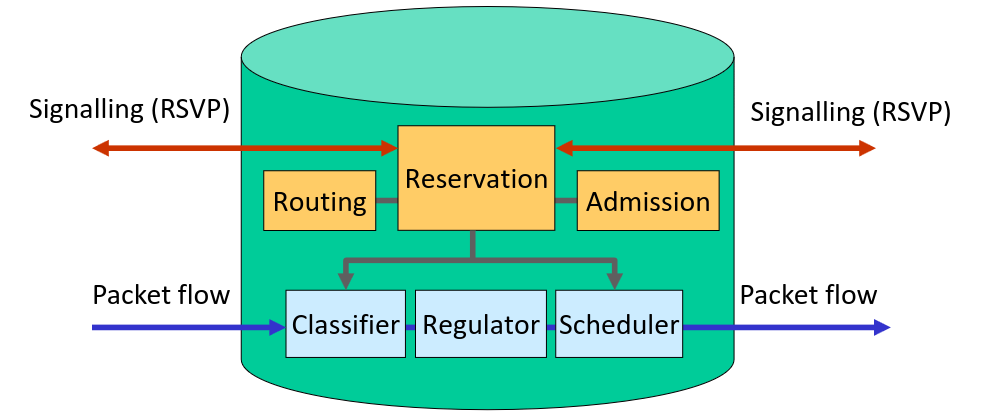
\includegraphics[width=0.5\textwidth]{pictures/5/router.png}
	\caption{Funzionalità dei router in IntServ}
\end{figure}
Il router dispone di:
\begin{itemize}
	\item \textbf{Signalling (RSVP)}
	\item \textbf{Routing}
	\item \textbf{Reservation}
	\item \textbf{Admission}
	\item \textbf{Packet flow}: Classifier, Regulator, Scheduler
\end{itemize}

\subsubsection{Classifier}
Identifica il flusso al quale appartiene il pacchetto in arrivo.

\subsubsection{Regulator}
Esegue la regolazione del traffico (policing/shaping/marking).

\subsubsection{Scheduler}
Seleziona il pacchetto da inviare per primo sul link di uscita.

\subsection{RSVP}
RSVP è un protocollo di livello 3, anche se utilizza gli stessi servizi di IP. I messaggi RSVP sono incapsulati in un pacchetto IP con Protocol ID 46. La congestione dei pacchetti di signalling deve essere limitata:
\begin{itemize}
	\item È necessario allocare una porzione di banda per il signalling.
	\item In alternativa, adozione di meccanismi di priorità.
\end{itemize}

\subsubsection{Prenotazione delle risorse}
RSVP è utilizzato per scambiare, per una data richiesta di prenotazione e sul percorso scelto, informazioni relative al QoS e alle risorse da riservare:
\begin{itemize}
	\item Ogni router valuta autonomamente se la richiesta può essere accettata.
	\item Se sì, memorizza le richieste accettate così che il QoS possa essere garantito una volta che i flussi di traffico correlati arrivano.
\end{itemize}

RSVP utilizza diversi messaggi, ma i più importanti sono PATH e RESV.

\subsubsection{Messaggio PATH}
Imposta il percorso su cui deve essere effettuata la prenotazione delle risorse:
\begin{itemize}
	\item È consegnato seguendo le regole standard di instradamento IP.
\end{itemize}

La sorgente invia un messaggio PATH alla destinazione:
\begin{itemize}
	\item I messaggi PATH sono inviati periodicamente per rilevare possibili cambi di routing.
	\item In tal caso, la prenotazione delle risorse deve essere effettuata nuovamente sul nuovo percorso.
\end{itemize}

Ogni router che riceve un messaggio PATH mantiene uno stato di percorso. Lo stato di percorso include:
\begin{itemize}
	\item L'indirizzo del nodo precedente (interfaccia) attraversato dal messaggio.
	\item Parametri caratteristici del flusso.
	\item L'interfaccia locale di ingresso e quella di uscita del messaggio PATH.
\end{itemize}

Lo stato di percorso è associato al flusso al quale il messaggio PATH si riferisce.

\subsubsection{Messaggio PATH: oggetti}
Il messaggio PATH include due oggetti fondamentali:
\begin{itemize}
	\item \textbf{TSPEC} (Traffic SPECification)
	\item \textbf{ADSPEC} (ADvertising SPECification, opzionale)
\end{itemize}

\subsubsection{TSPEC}
TSPEC rende possibile informare i router sulle caratteristiche del flusso. Contiene una descrizione del traffico generato dalla sorgente (tipicamente parametri di token bucket). TSPEC non può essere modificato dai router.

\subsubsection{ADSPEC}
Se incluso, ADSPEC raccoglie informazioni preliminari sul QoS che può essere garantito sul percorso. È esaminato e appropriatamente modificato ad ogni hop:
\begin{itemize}
	\item Sintetizza informazioni sul QoS ottenibile sul percorso.
	\item Ad es. se ci sono router non RSVP-compliant, se certe classi di servizio non sono supportate, quale è la banda minima che può essere garantita, ecc.
\end{itemize}

\subsubsection{Messaggio RESV}
La destinazione genera un messaggio RESV verso la sorgente per effettuare richieste di prenotazione. Il messaggio RESV percorre lo stesso percorso del messaggio PATH, ma in direzione opposta:
\begin{itemize}
	\item Il routing dei messaggi RESV non segue le regole di instradamento IP: è invece adottato il routing basato sulla sorgente.
	\item Le informazioni sul \textit{percorso inverso} sono portate dal corrispondente messaggio PATH.
\end{itemize}

In base ai campi TSPEC e ADSPEC (se incluso) ricevuti nel messaggio PATH, la destinazione determina quale richiesta di prenotazione deve essere effettuata.

\subsubsection{Messaggio RESV: FLOWSPEC}
Un oggetto fondamentale è incluso:
\begin{itemize}
	\item \textbf{FLOWSPEC} (FLOW SPECification)
\end{itemize}

FLOWSPEC specifica la prenotazione delle risorse da effettuare. Include il/i sub-oggetto/i TSPEC e (opzionalmente) RSPEC (Reservation SPECification):
\begin{itemize}
	\item \textbf{TSPEC}: include le caratteristiche del flusso, possibilmente modificate dalla destinazione.
	\item \textbf{RSPEC}: se incluso, contiene i parametri di QoS del tipo di servizio desiderato. Specifica le garanzie da offrire al traffico, come la banda dedicata richiesta.
\end{itemize}

\subsubsection{Messaggio RESV e Call Admission}
Il Call Admission è effettuato passo-passo dai router sul percorso quando il messaggio RESV è ricevuto. Ogni router:
\begin{enumerate}
	\item Riceve le informazioni di flusso [e QoS] come input (TSPEC [e RSPEC]).
	\item Conosce l'occupazione delle sue risorse dovuta ai flussi già accettati.
	\item Due casi:
	\begin{itemize}
		\item Accetta il nuovo flusso se possono essere allocate sufficienti risorse locali per garantire il QoS; determina un nuovo RSPEC da inviare a monte (se RSPEC è incluso).
		\item Altrimenti, rifiuta la richiesta (le risorse non sono riservate).
	\end{itemize}
\end{enumerate}

In caso di accettazione, il flusso è assegnato alle risorse di rete dedicate necessarie per soddisfare i requisiti di QoS. I parametri degli scheduler e dei classifier sono impostati. In caso contrario, viene effettuato il REJECT.
\begin{figure}[H]
	\centering
	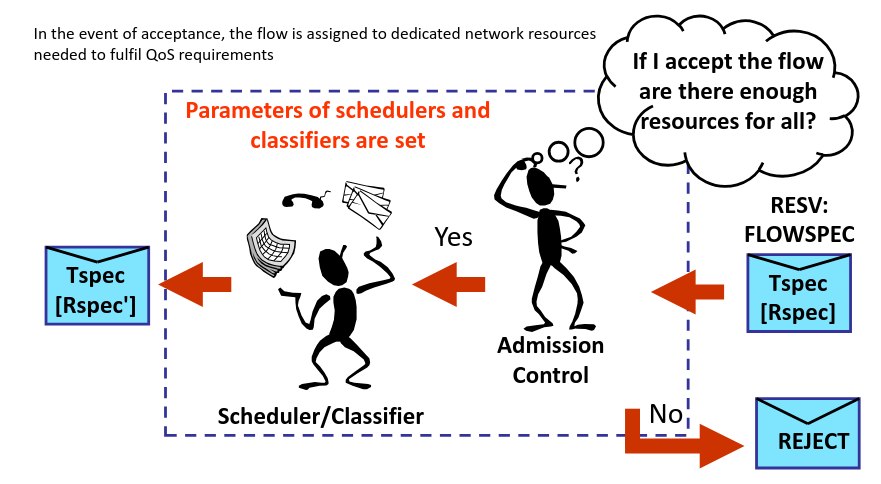
\includegraphics[width=0.8\textwidth]{pictures/5/rsvp.png}
\end{figure}

\subsection{RSVP e controllo del traffico}
I router di confine eseguono la regolazione del traffico (policing, shaping, marking) basandosi sui parametri dichiarati (portati nel messaggio RESV). I router core eseguono:
\begin{itemize}
	\item Classificazione dei pacchetti di ogni flusso.
	\item Regolazione del traffico.
	\item Scheduling basato sul QoS richiesto.
\end{itemize}

\subsection{RSVP – Soft state}
Lo soft state è lo stato mantenuto nei router che è limitato nel tempo e controllato da un timer. Sorgente e destinazione periodicamente scambiano nuovi messaggi PATH/RESV.

\textbf{Vantaggi}
\begin{itemize}
	\item Possibilità di recupero da situazioni di errore.
	\item Tolleranza alla perdita di pacchetti di signalling.
	\item Le risorse possono essere deallocate se un flusso non è più attivo nella rete.
	\item Buona adattabilità ai cambiamenti nel percorso tra sorgente e destinazione.
\end{itemize}

\textbf{Svantaggio}: aumento del traffico di signalling di rete.

\subsection{RSVP – Tutti i messaggi}
\begin{itemize}
	\item \textbf{PATH}: messaggio iniziale sul percorso in avanti.
	\item \textbf{RESV}: messaggio di prenotazione sul percorso all'indietro.
	\item \textbf{PATH ERR}: comunica l'identificazione degli errori durante l'elaborazione del messaggio PATH.
	\item \textbf{RESV ERR}: indica il fallimento della fase di prenotazione.
	\item \textbf{PATH TEAR}: abbatte lo stato stabilito nei router da un messaggio PATH.
	\item \textbf{RESV TEAR}: abbatte lo stato stabilito nei router da un messaggio RESV.
	\item \textbf{RESV CONF (opzionale)}: messaggio inviato alla destinazione per confermare il successo della fase di prenotazione delle risorse.
\end{itemize}

\subsection{Formato dei messaggi RSVP}
Un messaggio RSVP è composto da un header (64 bit) seguito da uno o più oggetti. La dimensione totale è un multiplo di 32 bit. Ogni oggetto include alcune informazioni specifiche portate dal messaggio:
\begin{itemize}
	\item Parametri di regolazione del traffico (ad es. TSPEC).
	\item Informazioni sul QoS ottenibile sul percorso (ad es. ADSPEC).
	\item \ldots
\end{itemize}

\subsection{Header del messaggio RSVP}
\begin{itemize}
	\item \textbf{Vers}: versione del protocollo (attualmente 1).
	\item \textbf{Flags}: attualmente non utilizzati.
	\item \textbf{Msg Type}: identificatore del tipo di messaggio (PATH, RESV, ecc.).
	\item \textbf{RSVP Checksum}: utilizzato per verificare l'integrità del messaggio.
	\item \textbf{Send\_TTL}: confrontandolo con il TTL dell'header IP, consente di rilevare che nodi non RSVP-compliant sono stati attraversati.
	\item \textbf{RSVP Length}: lunghezza del messaggio (in byte).
\end{itemize}

\subsection{Oggetti RSVP}
Ogni oggetto ha:
\begin{itemize}
	\item \textbf{Length}: lunghezza dell'oggetto (in byte).
	\item \textbf{Class\_NUM}: tipo di oggetto (ADSPEC, TSPEC, FLOWSPEC, ecc.).
	\item \textbf{C-Type}: tipo di formato utilizzato per un tipo di oggetto (1 IPv4, 2 IPv6, 7 MPLS, \ldots).
\end{itemize}

\subsection{Allocazione delle risorse}
Le risorse sono allocate da RSVP in modo diverso per le due classi di servizio supportate:
\begin{itemize}
	\item Guaranteed Service (GS).
	\item Controlled Load Service (CLS).
\end{itemize}

\subsection{Guaranteed Service (RFC 2212)}
Emula un servizio a circuito con ritardi garantiti. Assicura:
\begin{enumerate}
	\item Nessuna perdita.
	\item Un limite superiore al ritardo end-to-end sperimentato.
\end{enumerate}

\subsection{Guaranteed Service (RFC 2212) – dettagli}
TSPEC definisce le caratteristiche del traffico e contiene i parametri del token bucket (specificati dal mittente e possibilmente modificati dal ricevitore nel TSPEC di destinazione):
\begin{itemize}
	\item Token bucket size $k$ [bit].
	\item Token rate $r$ [bit/s].
	\item Peak rate $p > r$ [bit/s].
\end{itemize}

ADSPEC contiene parametri che permettono al ricevitore di stimare il ritardo end-to-end e la banda disponibile nella rete lungo il percorso scelto:
\begin{itemize}
	\item Banda minima disponibile.
	\item Ritardo minimo introdotto (somma dei ritardi per ogni link).
\end{itemize}

RSPEC (in FLOWSPEC) include i seguenti parametri:
\begin{itemize}
	\item Banda $B$ [bit/s] da riservare.
	\item Termine di slack (o termine di correzione) $S$ [$\mu$s].
\end{itemize}

\subsection{Guaranteed Service (RFC 2212) – workflow}
\begin{enumerate}
	\item Il ricevitore, basandosi su ADSPEC ricevuto (messaggio PATH), determina la banda $B_j$ da allocare dai router al flusso $j$ e il termine di slack $S$:
	\[
	S = \text{ritardo end-to-end tollerabile} - \text{ritardo end-to-end con prenotazione di banda } B_j
	\]
	\item Il ricevitore invia $B_j$ e $S$ in RSPEC (messaggio RESV):
	\begin{itemize}
		\item Se $S$ è positivo, i router a monte possono ridurre $B_j$ (e conseguentemente $S$), quindi aggiornare RSPEC, oppure non modificare questi valori.
		\item Se la banda $B_j$ non è disponibile in un router sul percorso e non può essere ridotta perché $S$ diventerebbe negativo, il flusso è rifiutato.
	\end{itemize}
\end{enumerate}

Questo meccanismo assicura che una porzione di banda $B_j$ sia riservata sul percorso e che il ritardo end-to-end non superi un dato valore massimo tollerato.

\subsection{Controlled Load Service (RFC 2211)}
Offre un servizio che emula best effort in una rete non congestionata:
\begin{itemize}
	\item Non garantisce un ritardo massimo.
\end{itemize}

La gestione sui nodi è più semplice rispetto al caso di Guaranteed Service:
\begin{itemize}
	\item Può essere implementata in molti modi diversi.
\end{itemize}

\subsection{Controlled Load Service (RFC 2211) – dettagli}
\begin{itemize}
	\item TSPEC contiene la descrizione dei parametri del token bucket (come nel caso di Guaranteed Service).
	\item ADSPEC (opzionale) non include alcuna informazione di ritardo e banda lungo il percorso: la banda disponibile e il ritardo end-to-end non sono stimati.
	\item FLOWSPEC non contiene RSPEC: ogni router prende decisioni localmente e indipendentemente rispetto alla banda $B_j$ che deve essere allocata al servizio.
\end{itemize}

\subsection{Integrated Services: problemi}
\begin{itemize}
	\item È necessario mantenere uno stato nei router per ogni flusso (sia per Guaranteed Service che per Controlled Load Service).
	\item Scarsa scalabilità.
	\item Signalling pesante.
	\item Forte impatto sull'architettura dei router.
	\item Adatto solo a reti piccole.
\end{itemize}
\section{Differentiated Services (DiffServ)}
Soluzione più semplice, scalabile e a costo inferiore rispetto a IntServ. Il controllo e la gestione flusso-per-flusso sono sostituiti nei router da una tecnica a grana grossa. Ogni classe di servizio è trattata collettivamente all'interno di ogni router:
\begin{itemize}
	\item Il QoS è garantito in termini relativi.
\end{itemize}

Può essere complementare e non alternativa a IntServ:
\begin{itemize}
	\item Le risorse possono comunque essere riservate a flussi individuali tramite RSVP se necessario.
\end{itemize}

\subsection{Nessun controllo sui micro-flows}
I micro-flows per ogni classe di servizio non sono gestiti individualmente. Qualsiasi traffico in eccesso per un micro-flow degrada il QoS di tutti i flussi appartenenti alla stessa classe di servizio. A livello di micro-flow è necessaria una strategia per la regolazione del traffico, come per IntServ:
\begin{itemize}
	\item Non specificato da DiffServ.
	\item Fondamentale (ancora più importante che per IntServ).
\end{itemize}

\subsection{Differentiated Services (RFC 2475)}
La regolazione del traffico a livello di micro-flow è effettuata esclusivamente ai bordi della rete (in edge router). I router interni (core routers) applicano soltanto il forwarding differenziato su pochi differenti traffici di classi di servizio:
\begin{itemize}
	\item Cambiamenti architetturali non significativi: sono richieste code diverse e algoritmi di scheduling, così come un meccanismo di classificazione.
	\item Non è necessario mantenere lo stato per ogni flusso.
\end{itemize}

\subsection{Differenziazione delle classi di servizio}
Il campo Differentiated Service (DS) dell'header IP è utilizzato per discriminare le diverse classi di servizio:
\begin{itemize}
	\item Corrisponde al byte TOS (Type of Service) di IPv4.
\end{itemize}

6 bit sono utilizzati per specificare il Differentiated Service Code Point (DSCP), mentre i rimanenti due bit non sono utilizzati:
\begin{itemize}
	\item DSCP è verificato per la classificazione.
	\item In base al DSCP viene scelto il tipo giusto di servizio (o Per-Hop Behaviour, PHB) da applicare al pacchetto dai router interni.
	\item Ad es. 0X00 indica il forwarding Best Effort.
\end{itemize}

\subsection{DiffServ nei router di bordo}
I router di bordo verificano la consistenza del traffico con SLA e TCA:
\begin{itemize}
	\item Il DSCP del pacchetto IP è definito (classificazione).
	\item La regolazione del traffico a livello di micro-flow è eseguita.
\end{itemize}

\subsection{DiffServ nei router core}
I router core gestiscono aggregati di traffico (ognuno correlato a una classe di servizio) e processano i macro-flows in base ai PHB selezionati:
\begin{itemize}
	\item Le condizioni locali (ad es. l'esistenza di congestione) possono influenzare il modo in cui i pacchetti sono processati.
\end{itemize}

\subsection{Per-Hop-Behaviour}
I Per-Hop-Behaviours (PHB) più importanti sono:
\begin{itemize}
	\item \textbf{Expedited Forwarding (EF)}: utilizzato per applicazioni che richiedono bassa latenza.
	\item \textbf{Assured Forwarding (AF)}: insieme di PHB utilizzati per applicazioni che richiedono garanzie di consegna.
	\item \textbf{Best Effort (BE)}: utilizzato per traffico senza alcuna garanzia.
\end{itemize}

\subsection{Expedited Forwarding (RFC 2598)}
Emulazione di una linea dedicata (servizio a circuito). Ritardi e percentuali di perdita di pacchetti devono essere molto bassi:
\begin{itemize}
	\item Il traffico deve essere condizionato e controllato.
	\item Il traffico in eccesso rispetto al TCA non è ammesso nella rete.
\end{itemize}

È il PHB a priorità più alta. DSCP: 101110.

\subsection{Assured Forwarding (RFC 2597)}
Fornisce quattro diversi livelli di priorità (cioè, classi) in termini di banda e allocazione delle code:
\begin{itemize}
	\item Quattro code diverse.
\end{itemize}

Cerca di evitare la congestione per mezzo di un drop differenziato e precoce dei pacchetti:
\begin{itemize}
	\item Tre diverse probabilità di scarto (cioè, livelli) per ciascuna delle quattro classi di priorità definite sopra.
\end{itemize}

\subsection{Assured Forwarding (RFC 2597) – scarto controllato}
Lo scarto dei pacchetti da parte dello scheduler avviene in modo controllato. Una semplice strategia di Tail Drop dovrebbe essere evitata:
\begin{itemize}
	\item Scarto incontrollato quando la coda è piena.
	\item Molto dannoso per il traffico che richiede basse perdite.
\end{itemize}

Una possibilità è di utilizzare l'algoritmo Random Early Discard (RED). Due diverse soglie per ogni livello in ogni classe determinano tre diverse aree di probabilità di scarto per ogni livello in ogni classe.

\subsection{Random Early Discard}
Assumendo che la classe AF sia fissata, ci sono tre diverse coppie $\{$min\_th$_i$, max\_th$_i\}$ (con $i=1,2,3$):
\begin{itemize}
	\item Una per ogni livello di probabilità di scarto $i$.
\end{itemize}

A seconda dell'occupazione della coda si hanno diverse aree di probabilità di scarto. Diversi valori massimi di probabilità di scarto nella zone di ``probabilità di scarto'' sono possibili.
\begin{multicols}{2}

\begin{figure}[H]
	\centering
	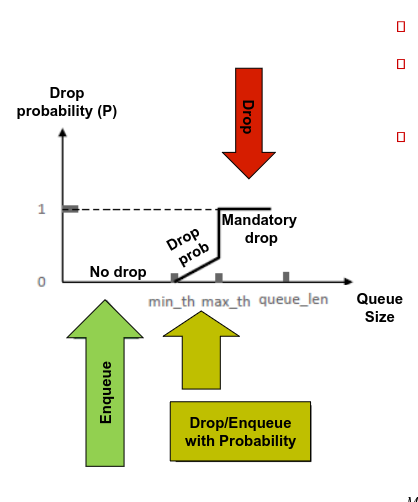
\includegraphics[width=0.4\textwidth]{pictures/5/randomearlydiscard1.png}
\end{figure}
\vfill
\begin{figure}[H]
	\centering
	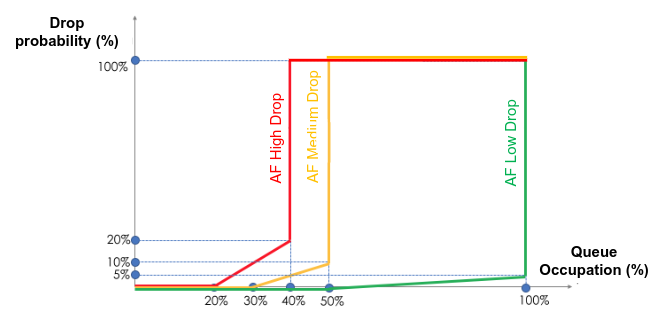
\includegraphics[width=0.5\textwidth]{pictures/5/randomearlydiscard2.png}
\end{figure}
\end{multicols}